\section*{Assignment 02: Network Effects and Launch Strategy}
\addcontentsline{toc}{section}{Assignment 02: Network Effects and Launch Strategy}

\subsection*{How we engineered the loops}
SkillSync only works if the student and organisation sides keep nudging each other into motion, so we mapped the network effects explicitly rather than hoping they appear by magic. The cross-side loop is the obvious one: more vetted NGO projects attract students hunting for impact portfolios; strong student turnout convinces resource-strapped organisations to post again. We layer two supportive loops on top. First, a same-side effect on the student side driven by peer stories, leaderboard shout-outs, and cohort-based feedback rituals that make participation feel communal \citep{Choudary2016}. Second, a data network effect where every completed match enriches our skill taxonomy and matching algorithm, pushing us closer to the curated-orchestrator archetype described by \citet{Reillier2017}.

\subsection*{Breaking the penguin problem}
The penguin problem hit us hard: no student wants to join before credible projects show up, yet NGOs hesitate without proven talent. We attacked it in three coordinated moves. Step one was to partner with two anchor NGOs who already mentored students informally; their endorsements provided the social proof \citet{HagiuWright2013} say you need to seed a young platform. Step two was to recruit a ``founding cohort'' of 40 students via faculty recommendations and give them concierge onboarding, stipends for the first deliverables, and a Slack space moderated by us. Step three layered lightweight guarantees: projects launched with pre-filled briefs, and we promised replacement support if a match fizzled. These subsidies mirror the playbooks from \citet{Gunasilan2024} and \citet{FarrellSaloner1986} on reducing switching risk when nobody wants to move first.

\subsection*{Launch strategy reflections}
Looking back, our soft launch favoured breadth over intensity. We opened the waitlist broadly and then scrambled to curate projects, which diluted the feeling of a vibrant community. If we reran it, I would narrow the first wave to one faculty and a handful of NGOs, mirroring the focused-cluster approach advocated by \citet{Choudary2016}. I would also front-load measurement on time-to-first-value and project completion rate so we react faster when loops drag \citep{ShapiroVarian1999}. Finally, we would invest earlier in student ambassadors embedded in each programme; when network effects rely on trust, credible peer voices beat email blasts every time.

Figure~\ref{fig:application-flow} captures the application flow that held those loops together. The screen-by-screen walkthrough shows how students browse curated projects, submit a tailored pitch, and immediately see the status of their application. We intentionally removed everything resembling a ``post and pray'' UX because that encourages low-effort spam that erodes quality. The step indicators at the top convey progress, while the embedded guidance chips reuse language from our mentoring sessions so the tone stays human.

\begin{figure}[h]
  \centering
  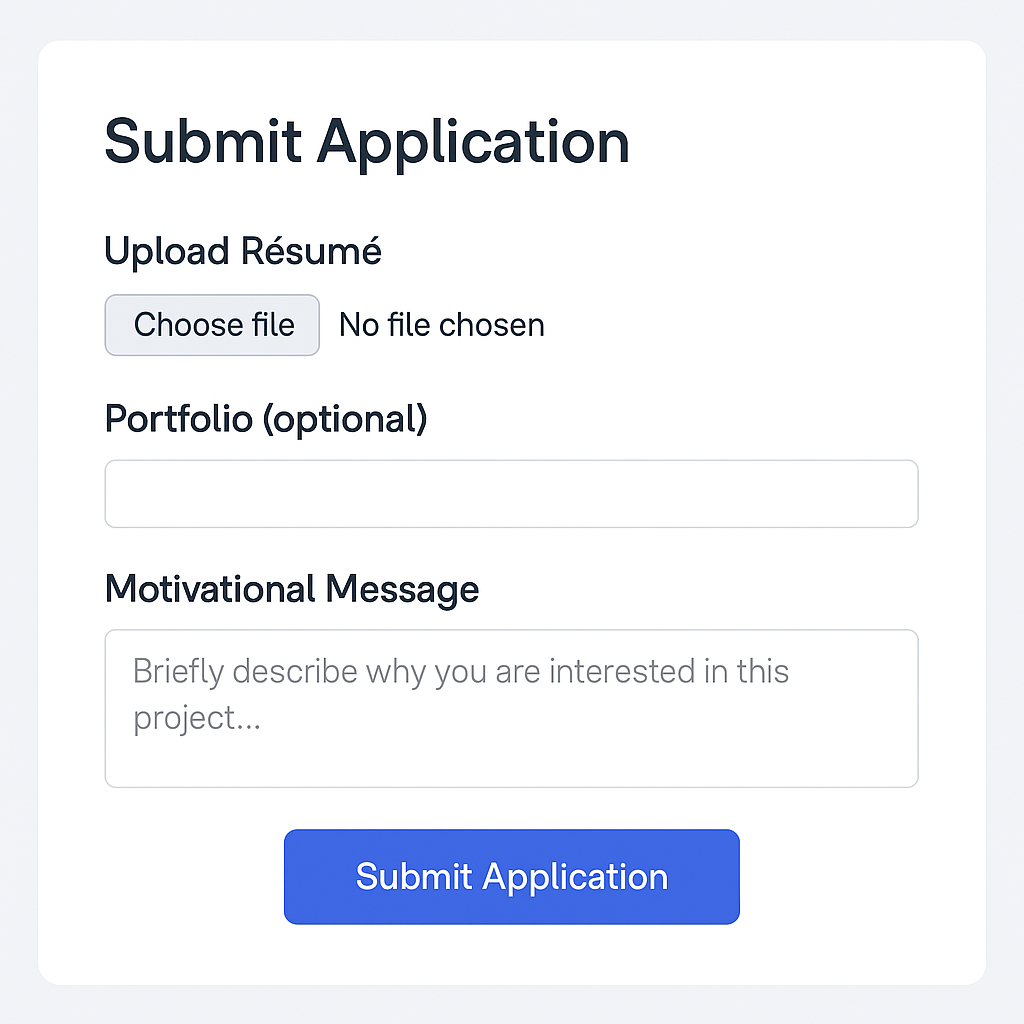
\includegraphics[width=0.85\linewidth]{ansoegningsflow.png}
  \caption{End-to-end student application flow (`ansoegningsflow.png`) used to trigger the first successful loops.}
  \label{fig:application-flow}
\end{figure}

I also revisited the organisational journey once the first dozen projects wrapped up. Figure~\ref{fig:project-creation} (embedded in Assignment~3) reveals how we embedded scoping prompts into the creation wizard so NGOs never submit half-baked briefs. Behind the scenes we set up Zapier automations that alert the founding cohort whenever a new project drops, which helped push acceptance time under 24 hours. In hindsight we should have built that automation sooner; the metrics in Assignment~08 show how delay kills repeat usage. Documenting it now makes the lesson explicit: seeding is as much about choreography and tooling as it is about subsidies.
